% Generated by tools/paper/render.py from main_text.py; edit the source there, not this file.
\section{Methods}

\subsection{Overview}

Each pair is assigned to an algorithm (Table~\ref{tab:engines}; Fig.~\ref{fig:overview}). Unit costs follow A*PA2 \citep{GrootKoerkamp2024astarpa2}: band doubling over 256-column tiles of bit-parallel words, pruned on long pairs by the gap-chaining seed heuristic \citep{GrootKoerkamp2024astarpa}, with near-identical pairs aligned by diagonal transition alone. Gap-affine costs use the wavefront of WFA and BiWFA \citep{MarcoSola2021wfa,MarcoSola2023biwfa}. At unit costs, diagonal transition runs first and hands over once its projected remaining work exceeds the band's and it has spent a twenty-fourth of the band's least work (Section 3.10); its projection, the length and the cost model then choose the next algorithm and its parameters.

At unit, gap-affine and two-piece costs, every engine selects the same alignment among equally good ones, by the backtrace order of WFA2-lib: from the end, an edit into a cell is preferred to a match whenever one is optimal, a substitution before a deletion (a letter of \(A\) alone) before an insertion (a letter of \(B\) alone), the second gap piece before the first, and a gap extended before it is opened. This rule gives WFA2-lib's CIGARs exactly; the default applies it to both sequences reversed, which places every edit as far left as possible, as variant callers normalise indels. The wavefronts and the tile traceback (Section 3.4) take the furthest-reaching source, which makes the same choice, and the batches and the difference sweep store per-cell flags under the rule. Two exceptions remain: a gap-affine pair whose wavefronts would exceed the memory limit is split and follows the rule within each piece, and alignments under a substitution matrix follow the traceback order of Gotoh's recurrence.

% Generated by tools/paper/render.py from main_text.py; edit the source there, not this file.
\begin{figure*}[t]
\centering
\resizebox{\textwidth}{!}{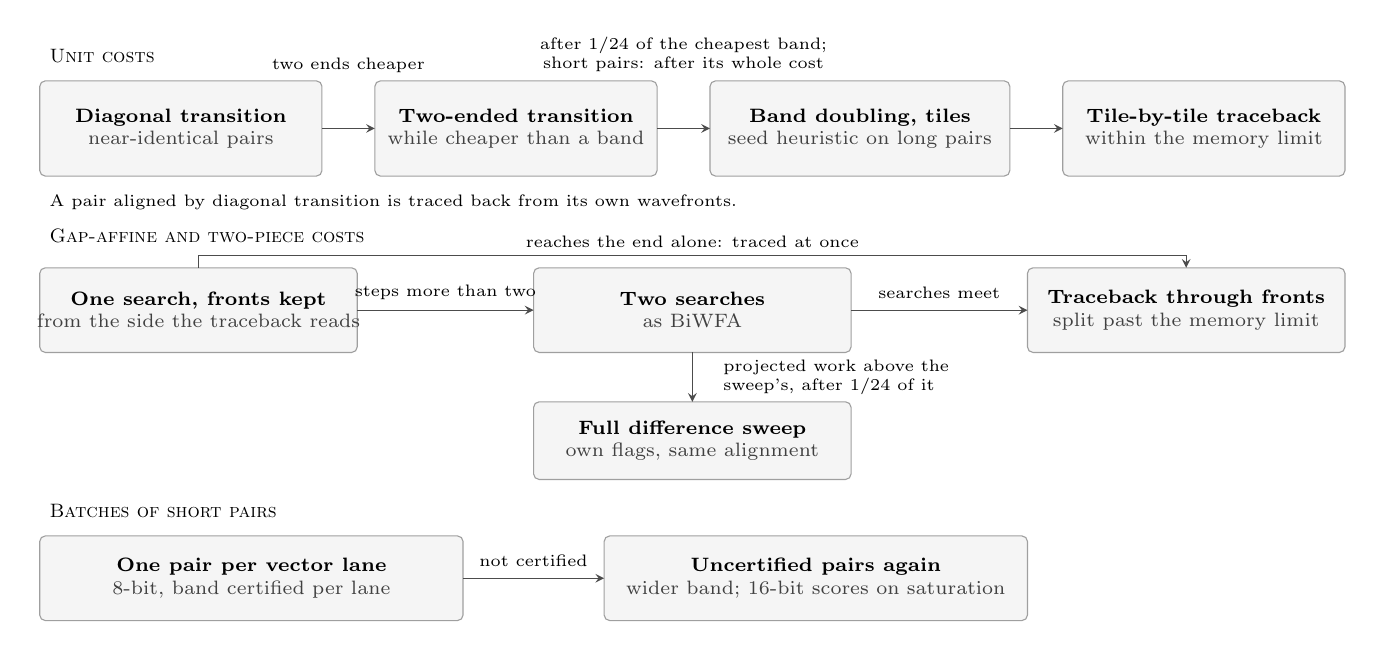
\begin{tikzpicture}
\node[anchor=west,font=\scriptsize\scshape] at (0.224,-0.224) {Unit costs};
\node[anchor=west,font=\scriptsize\scshape] at (0.224,-2.509) {Gap-affine and two-piece costs};
\node[anchor=west,font=\scriptsize\scshape] at (0.224,-6.003) {Batches of short pairs};
\draw[rounded corners=2pt,fill=gray!8,draw=gray!75] (0.224,-0.538) rectangle (3.808,-1.747);
\node[align=center,font=\scriptsize] at (2.016,-1.142) {\textbf{Diagonal transition}\\{\color{black!75}near-identical pairs}};
\draw[rounded corners=2pt,fill=gray!8,draw=gray!75] (4.480,-0.538) rectangle (8.064,-1.747);
\node[align=center,font=\scriptsize] at (6.272,-1.142) {\textbf{Two-ended transition}\\{\color{black!75}while cheaper than a band}};
\draw[rounded corners=2pt,fill=gray!8,draw=gray!75] (8.736,-0.538) rectangle (12.544,-1.747);
\node[align=center,font=\scriptsize] at (10.640,-1.142) {\textbf{Band doubling, tiles}\\{\color{black!75}seed heuristic on long pairs}};
\draw[rounded corners=2pt,fill=gray!8,draw=gray!75] (13.216,-0.538) rectangle (16.800,-1.747);
\node[align=center,font=\scriptsize] at (15.008,-1.142) {\textbf{Tile-by-tile traceback}\\{\color{black!75}within the memory limit}};
\draw[rounded corners=2pt,fill=gray!8,draw=gray!75] (0.224,-2.912) rectangle (4.256,-3.987);
\node[align=center,font=\scriptsize] at (2.240,-3.450) {\textbf{One search, fronts kept}\\{\color{black!75}from the side the traceback reads}};
\draw[rounded corners=2pt,fill=gray!8,draw=gray!75] (6.496,-2.912) rectangle (10.528,-3.987);
\node[align=center,font=\scriptsize] at (8.512,-3.450) {\textbf{Two searches}\\{\color{black!75}as BiWFA}};
\draw[rounded corners=2pt,fill=gray!8,draw=gray!75] (12.768,-2.912) rectangle (16.800,-3.987);
\node[align=center,font=\scriptsize] at (14.784,-3.450) {\textbf{Traceback through fronts}\\{\color{black!75}split past the memory limit}};
\draw[rounded corners=2pt,fill=gray!8,draw=gray!75] (6.496,-4.614) rectangle (10.528,-5.600);
\node[align=center,font=\scriptsize] at (8.512,-5.107) {\textbf{Full difference sweep}\\{\color{black!75}own flags, same alignment}};
\draw[rounded corners=2pt,fill=gray!8,draw=gray!75] (0.224,-6.317) rectangle (5.600,-7.392);
\node[align=center,font=\scriptsize] at (2.912,-6.854) {\textbf{One pair per vector lane}\\{\color{black!75}8-bit, band certified per lane}};
\draw[rounded corners=2pt,fill=gray!8,draw=gray!75] (7.392,-6.317) rectangle (12.768,-7.392);
\node[align=center,font=\scriptsize] at (10.080,-6.854) {\textbf{Uncertified pairs again}\\{\color{black!75}wider band; 16-bit scores on saturation}};
\draw[->,>=stealth,black!70] (3.808,-1.142) -- (4.480,-1.142);
\node[align=center,font=\fontsize{6}{7}\selectfont] at (4.144,-0.336) {two ends cheaper};
\draw[->,>=stealth,black!70] (8.064,-1.142) -- (8.736,-1.142);
\node[align=center,font=\fontsize{6}{7}\selectfont] at (8.400,-0.202) {after 1/24 of the cheapest band;\\short pairs: after its whole cost};
\draw[->,>=stealth,black!70] (12.544,-1.142) -- (13.216,-1.142);
\draw[->,>=stealth,black!70] (4.256,-3.450) -- (6.496,-3.450);
\node[align=center,font=\fontsize{6}{7}\selectfont] at (5.376,-3.226) {steps more than two};
\draw[->,>=stealth,black!70] (10.528,-3.450) -- (12.768,-3.450);
\node[align=center,font=\fontsize{6}{7}\selectfont] at (11.648,-3.226) {searches meet};
\draw[->,>=stealth,black!70] (2.240,-2.912) -- (2.240,-2.755) -- (14.784,-2.755) -- (14.784,-2.912);
\node[align=center,font=\fontsize{6}{7}\selectfont] at (8.512,-2.576) {reaches the end alone: traced at once};
\draw[->,>=stealth,black!70] (8.512,-3.987) -- (8.512,-4.614);
\node[anchor=west,align=left,font=\fontsize{6}{7}\selectfont] at (8.781,-4.301) {projected work above the\\sweep's, after 1/24 of it};
\draw[->,>=stealth,black!70] (5.600,-6.854) -- (7.392,-6.854);
\node[align=center,font=\fontsize{6}{7}\selectfont] at (6.496,-6.630) {not certified};
\node[anchor=west,font=\fontsize{6}{7}\selectfont] at (0.224,-2.083) {A pair aligned by diagonal transition is traced back from its own wavefronts.};
\end{tikzpicture}}
\caption{How dinara-align assigns a pair to an algorithm, and the rule behind each hand-over. At unit costs, diagonal transition from one end and then from both aligns near-identical pairs, switching to both ends once they would finish more cheaply and handing over to band doubling over bit-parallel tiles only once its projected work exceeds the band's and it has spent one twenty-fourth of the cheapest band, or, for a pair of at most 2{,}048 columns, whose band covers the whole matrix, only once it has spent that band's whole cost (Section 3.10); the tiles are traced back within the memory limit. At gap-affine costs one search grows alone, its fronts kept, and is traced back at once if it reaches the end; a second search joins once one would step more diagonals than two would need (Section 3.9), and a global pair projected to take more work than a full sweep in difference recurrences is handed to that sweep after one twenty-fourth of its work, the alignment the same either way. Batches of short pairs are aligned one pair per vector lane within a band whose optimality each lane certifies (Section 3.6). The figure shows alignments; a unit-cost distance skips the one-ended search.}\label{fig:overview}
\end{figure*}


% Generated by tools/paper/render.py from main_text.py; edit the source there, not this file.
\begin{table*}[t]
\caption{Algorithms in dinara-align and the changes introduced in this work.}\label{tab:engines}
\centering\footnotesize
\setlength{\tabcolsep}{4pt}
\begin{tabular}{@{}l>{\raggedright\arraybackslash}p{5.2cm}>{\raggedright\arraybackslash}p{5.2cm}@{}}
\toprule
Problem & Algorithm & Changes (section) \\
\midrule
Unit costs, divergent pairs & Band doubling over bit-parallel tiles with the gap-chaining seed heuristic (A*PA2) & Regrouped recurrence, interleaved groups (3.2); agreeing estimates (3.3); direct neighbours (3.5); traceback within a memory limit (3.7) \\
Unit costs, near-identical pairs & Diagonal transition (WFA, BiWFA) & Gathered extension (3.4); estimate-delayed hand-over (3.10); per-pair overhead (3.11) \\
Gap-affine, two-piece & Wavefront, one search or two (WFA, BiWFA); full sweep in difference recurrences for divergent pairs (Suzuki and Kasahara, 2018) & Gathered extension (3.4); one search or two (3.9); estimate-delayed hand-over (3.10) \\
Substitution matrices & Anti-diagonal vector sweep (Wozniak, 1997) & Score-certified band, cache-sized strips (3.8) \\
Local alignment & End found by a forward sweep (Zhao et al., 2013) & Backward wavefront from the best end (3.8) \\
Batches of short pairs & Inter-sequence vectorisation (Rognes, 2011; Rahn et al., 2018; Daily, 2016) & Certified per-lane bands (3.6) \\
\bottomrule
\end{tabular}
\end{table*}


\subsection{A shorter critical path for Myers' recurrence}

As in Edlib and A*PA2 \citep{Sosic2017edlib,GrootKoerkamp2024astarpa2}, the query is packed 64 bases per word, and Myers' recurrence \citep{Myers1999bitvector} advances a word by one column. With match mask \(E\), vertical difference masks \(P_v, M_v\) and the incoming negative horizontal difference folded into \(E' = E \lor M_h^{\mathrm{in}}\), A*PA2 computes

\begin{equation}\begin{gathered}
c = (E' \land P_v) + P_v,\\ X_h = (c \oplus P_v) \lor E',\\ P_h = M_v \lor \lnot(X_h \lor P_v),\\ M_h = P_v \land X_h.
\end{gathered}\end{equation}

The horizontal masks \(P_h\) and \(M_h\) determine the vertical masks of the next column, so the path from \(c\) to them lies on the loop-carried chain. Since \((c \oplus P_v) \lor P_v = c \lor P_v\) and \(P_v \land (c \oplus P_v) = P_v \land \lnot c\), the same masks are obtained as

\begin{equation}\begin{gathered}
P_h = M_v \lor \lnot\bigl(c \lor (E' \lor P_v)\bigr),\\ M_h = (P_v \land \lnot c) \lor (P_v \land E'),
\end{gathered}\end{equation}

where \(E' \lor P_v\) and \(P_v \land E'\) do not depend on \(c\) and are computed off the critical path. The vertical update is regrouped in the same way, its negated part computed from \(E\), \(M_v\) and the incoming horizontal difference before \(P_h\) is known. Together the rewrites shorten the loop-carried chain of a single word from 14 to 8 cycles per column. \citet{Myers1999bitvector}, Edlib and A*PA2 use the original form, and we are not aware of a previous description of the regrouped one.

Words occupy the lanes of a vector, staggered by one column, so that the horizontal difference leaving one word enters the next through a lane rotation \citep{Wozniak1997,GrootKoerkamp2024astarpa2}, and each column waits for the rotation of the previous one. A*PA2 overlaps these waits with two four-lane vectors; on AVX-512, where a vector holds eight words, dinara-align interleaves two eight-word groups, the lower ten columns behind the upper, so that each fills the latency of the other. Bands of two or three words run in general-purpose registers, whose operations have lower latency.

\subsection{Band bounds from agreeing estimates}

Band doubling is exact for any initial bound, but its running time depends on how close that bound is to the distance. A computation that has reached cost \(s\) at anti-diagonal \(\rho\) estimates the distance as \(\hat D = s(n+m)/\rho\), which is reliable when edits are spread evenly and too high by orders of magnitude when they gather, as at the ends of nanopore reads. dinara-align therefore takes two estimates, \(\hat D_1\) from a one-ended diagonal-transition search stopped after eight edits and \(\hat D_2\) from the two-ended search where it handed over. When at least one seed in 32 chains from the origin, the first bound starts 64 above the seed heuristic there, which on long reads lies within a few per cent of the distance. Otherwise it is aimed just above \(\hat D_1\) when \(\max(\hat D_1,\hat D_2) \le \tfrac43 \min(\hat D_1,\hat D_2)\) or the search stopped within 16 edits, and failing both, as in A*PA2, it starts at most 256 above the known lower bound and each retry at most doubles it until a failed round has crossed one eighth of the columns, far enough for where it stopped to estimate the distance. A failed round aims the next bound from where it stopped, and the first round estimates the distance again after one eighth, one quarter and one half of the columns, lowering its bound or abandoning the round. A distance is accepted only within the bound its round ended on, and these rules change only the sequence of bounds, so the result stays exact.

Within a round, the band drops the rows at the top and bottom of each tile whose score plus the heuristic exceeds the bound, as A*PA2 does. A score changes by at most one per row, and the heuristic by at most its climb \(\gamma\) (one without seeds or with exact seeds, two with inexact ones), so a row that exceeds the bound by \(y\) rules out itself and the next \(\lceil y/(1+\gamma) \rceil - 1\) rows, which are skipped unread.

\subsection{Diagonal transition for near-identical pairs}

Diagonal transition extends each diagonal of a wavefront along its run of matches. dinara-align compares eight letters at a time by the exclusive-or of two 64-bit words and a count of trailing zeros, and on AVX-512 extends eight diagonals together, their letters loaded by gather instructions under branch-free masks (Supplementary Section S1.1). The same vectorised step serves three uses: near-identical pairs, from one or both ends \citep{MarcoSola2023biwfa}; the traceback inside each tile, restricted to the diagonals that can still reach the traced cell; and the three-layer gap-affine front.

A pair that diagonal transition finishes before handing over is aligned from its wavefronts alone. From both ends, as in BiWFA, the forward wavefronts are grown on to the proven distance, each cost kept only on the diagonals on which the backward wavefronts show that an optimal path passes. The backtrace takes the furthest-reaching source at each cost (Section 3.1) and writes the CIGAR run by run.

\subsection{Seed heuristic: direct neighbour construction}

The reference is divided into disjoint seeds of 12 bases, matched exactly, or of 16 bases, matched with at most one edit \citep{GrootKoerkamp2024astarpa}; a 16-base seed matched with one edit matches one of its 8-base halves exactly, so each half indexes a table. The lookups for 16 query rows are issued together, so that their cache misses overlap, and only seeds whose matches could still chain to the end of the pair are considered.

An exact match \(\mu\) of a 16-base seed at query rows \([j, j+16)\) has four neighbouring matches with one edit, fewer at the ends of the query: two share its start, at rows \([j, j+15)\) and \([j, j+17)\), and two share its end, at \([j+1, j+16)\) and \([j-1, j+16)\). Because chaining is all-or-nothing, a neighbour one diagonal away may chain where \(\mu\) cannot, and the neighbours are required for the heuristic to remain a lower bound. Rather than locating them by search and testing each for local pruning, dinara-align inserts them whenever \(\mu\) is retained, which is justified by the following lemma, in which the search is the diagonal transition of local pruning (Section 2.4).

\textbf{Lemma 1.} If the search from an exact match \(\mu\) finds no path across the next \(p\) seeds, it finds none from any of its four neighbours.

\emph{Proof idea.} The search from \(\mu\) dominates that from each neighbour: at every cost and on every diagonal it reaches at least as far, and a further point has crossed at least as much potential, so it is dropped only if the nearer one is too (proof in Supplementary Section S6).

Every neighbour that the search would keep is therefore inserted. As in A*PA2, the implementation also keeps a match whose search runs into the start of a match already kept on the same diagonal, which keeps more matches and drops none. A match is thus dropped only if its search would find no path: either the search ran and found none, or the match neighbours an exact match whose search found none (Lemma 1). Dropping such matches keeps the heuristic a lower bound (Lemma S1), and each further match kept can only lower it, so the alignment stays exact. Each neighbour is placed in its layer from its own end's chain, without a search of its own.

\subsection{Certified bands for inter-sequence batches}

Batches of short pairs are aligned with one pair per vector lane \citep{Rognes2011swipe,Rahn2018seqan} in saturating 8-bit lanes \citep{Zhao2013ssw,Daily2016parasail}; a score that saturates is computed again in 16-bit lanes, and an alignment that saturates goes to the single-pair engines. Rather than computing each matrix in full, the lanes of a group compute the band of diagonals \([d_\ell, d_h]\) containing the main diagonal 0 and each pair's end diagonal \(\delta\), with one further diagonal on either side; pairs are grouped by end diagonal, so the band stays narrow. Its optimality is certified by the following bound, a cost form of the out-of-band bounds of \citet{Gibrat2018band} and \citet{Fujiki2020seedex} for gap-affine and two-piece costs, with a strict form for tie-breaking.

\textbf{Proposition 1.} Let \(C\) be the least cost of an alignment within \([d_\ell, d_h]\), and let \(L(d) = g(|d|) + g(|d-\delta|)\), or \(\infty\) for a diagonal outside the matrix. If \(C \le \min\bigl(L(d_h+1), L(d_\ell-1)\bigr)\), then \(C\) is the optimal cost; if the inequality is strict, every optimal alignment lies within the band.

\emph{Proof idea.} An alignment that leaves the band must open a gap reaching the diagonal beyond it and another returning to the end diagonal, which together cost at least \(L(d)\) for that diagonal \(d\) (proof in Supplementary Section S6).

Each vector lane of an inter-sequence batch evaluates its own certificate. When every optimal alignment lies in the band, each in-band score on an optimal path is exact, so the tie rule makes the same choices as in the full matrix, and the strict form guarantees that the alignment it selects lies within the band. Pairs that fail are recomputed over every diagonal that a path at most as cheap could visit, grouped by power-of-two classes of that band's width so that the lanes of a group finish together.

\subsection{Traceback within a memory limit}

The traceback of a band traces each tile from the boundary recorded on its left. On 1~Mbp pairs at 20\% errors, keeping every boundary made an alignment grow peak memory by up to 175 MiB, so the boundaries are held within the alignment's memory limit, 80 MiB by default: beyond it only one boundary in two is kept, then one in four, and so on. Each tile also records the state the band carries into it, from which the traceback recomputes a stretch of tiles starting at the last kept boundary (Supplementary Section S1.1). Every step of a band depends only on this state and on the scores it computes, so each boundary is recovered as the round left it and the alignment is the same byte for byte; splitting the pair instead, as QuickEd does \citep{Doblas2025quicked}, resolves ties within each part. On the 1~Mbp pairs at 20\% errors, the growth of peak memory fell from 175 to 133 MiB on the worst pair when this was introduced, for 9\% more time; Section 4.2 gives the figure at the reported commit.

\subsection{Gap-affine and score-based alignment}

A scoring scheme with match score \(\alpha\), mismatch score \(\beta\) and gap scores \(-(o+ke)\) can be converted into costs for global alignment \citep{Eizenga2022wfalm}. Every alignment covers \(n+m\) letters, so its score \(S\) and a gap-affine cost \(C\) satisfy

\begin{equation}\begin{gathered}
S = \tfrac12\bigl(\alpha(n+m) - C\bigr),\\ C = 2(\alpha-\beta)\,X + \sum_{\text{gaps}} \bigl(2o + k(2e+\alpha)\bigr),
\end{gathered}\end{equation}

where \(X\) is the number of mismatches, so the wavefront computes score-maximising alignments. Local alignment locates the end of the optimal alignment with a forward sweep, as in SSW \citep{Zhao2013ssw}, and extends a wavefront back from it to the first cell attaining the maximal score, which avoids the correction pass that striped layouts may need \citep{Farrar2007striped}.

The wavefront keeps five bytes per diagonal for the traceback, and a pair whose fronts would exceed the memory limit is split where an optimal path crosses, as in BiWFA, following the tie rule within each piece (Section 3.1). A global pair projected to take more work than a full sweep in 8-bit difference recurrences \citep{Suzuki2018diff} is handed to that sweep (Section 3.10), which keeps the predecessor flags of Section 3.1; unrelated 5~kbp pairs then aligned in 4.8~ms instead of 32.9~ms.

Under a substitution matrix, anti-diagonals \citep{Wozniak1997} are computed in 16-bit lanes while the scores provably fit, in strips of rows that stay in the first-level cache, and a global alignment is traced in a band of diagonals that grows until its own score proves that every optimal path lies inside it (Supplementary Section S1.4).

\subsection{One search or two at gap-affine costs}

WFA grows the wavefront from one end of the pair and keeps every front for the traceback \citep{MarcoSola2021wfa}; BiWFA grows it from both ends and keeps only the latest fronts \citep{MarcoSola2023biwfa}. Two searches must also prove where an optimal path crosses between them, so they stop only once \(2\min(s_1, s_2) \ge C^* - 1 + \theta\), where \(s_1, s_2\) are their costs, \(C^*\) the cheapest meeting found and \(\theta = o + w\) a margin: \(o\) is the largest gap-open cost and \(w = \max(x, o+e)\) the largest cost of a single edit, over both pieces for two-piece costs. Every optimal path has a cell whose costs from the two ends differ by at most \(w\), and a meeting inside a gap pays its opening once for both halves; BiWFA stops by the same margin. A score-only computation, which needs no meeting cell, stops sooner: once its best is at most one more than the highest cost to which either search has checked the other's start. With \(W(s)\) the number of diagonals a search steps to reach cost \(s\), two searches need about \(2W((C_{\mathrm{opt}}+\theta)/2)\) steps for a pair of cost \(C_{\mathrm{opt}}\), plus the setup of the second, and one search \(W(C_{\mathrm{opt}})\). Where the fronts widen with the cost, \(W(s)\) grows with \(s^2\) and one search is cheaper while \(C_{\mathrm{opt}} < (1+\sqrt2)\,\theta\); where the ends of the sequences bound the fronts, it is always cheaper. Most 250~bp Illumina reads cost less than \(\theta\) (14 at (4, 6, 2)), and on them two searches took 2.82~\textmu s per read in the benchmark runner, against 1.55~\textmu s for WFA.

dinara-align therefore starts with a single search, the one whose fronts the traceback reads (the backward search under the default tie rule), keeps its fronts and traces the alignment as soon as the search reaches the far corner. Every cost \(s\) passed without reaching it shows that \(C_{\mathrm{opt}} > s\), and the search measures \(W\) as it grows: it continues alone while \(s < \theta\), costs the second search would pass in any case, and then while \(W(s) \le 2W(\lfloor (s+\theta)/2 \rfloor)\), that is, while it has stepped no more diagonals than two searches would need for the cheapest cost still possible. It also hands over at half the memory limit or when a band leaves it no reachable cell. The rule has no tuned constant: it hands over at about \(2.4\theta\) where the fronts widen with the cost, and never where the sequences bound the fronts from early costs on, where it aligns exactly as WFA does.

\textbf{Proposition 2.} Suppose the first search stops at cost \(\sigma\) without reaching the far corner, and the second search, growing from cost 0, checks each new front against the last \(w+1\) fronts of the first, costs \(\sigma-w\) to \(\sigma\), while its own cost is at most \(\sigma\), after which the two alternate as in BiWFA, each new front checked against the other side's last \(w+1\). When they stop, \(C^*\) is the optimal cost and its meeting lies on an optimal path.

\emph{Proof idea.} On every optimal path the costs from the two starts change by at most \(w\) a move, so some cell has them within \(w\) of each other, and the two phases check every such cell before the stopping rule can end the searches (proof in Supplementary Section S6).

An alignment traced from the unpruned fronts of the single search is the one the two searches would have traced: the traceback steps only from a cell to a predecessor on an optimal path, and the fronts that two searches prune hold no such cell, so the tie rule is unchanged. Starting with one search took a 250~bp Illumina read at (4, 6, 2), through one aligner, from 2.41 to 1.52~\textmu s, and the measured-work rule, in place of a single search that grew alone only through its first \(w\) costs, saved a further 5\%, a third on the pairs costing 9 to 32; nanopore and HiFi reads were unchanged.

\subsection{Hand-overs that wait on a runtime estimate}

Two hand-overs rest on projections, the work still needed extrapolated from the edits seen so far: diagonal transition hands over to band doubling once its remaining work is projected to exceed a band's, and the gap-affine wavefront to the difference sweep once its projected total exceeds the sweep's. A projection is reliable when edits are spread evenly, but can exceed the distance a hundredfold when they gather at the ends, as on nanopore reads with adapters or poly-A tails, and so hand a pair that the search would finish in microseconds to a band over the whole matrix. dinara-align hands over on a projection only once the work already spent has reached one twenty-fourth of the cheapest alternative that could still be needed: for diagonal transition, the band whose bound equals the cost already reached, which no band can undercut since the distance is at least that cost; for the wavefront, the full sweep. Once the projection favours the alternative, the rule thus delays the hand-over by at most about 4\% (1/24, in the units of the cost model) of the work the alternative needs in any case, while a search that would have finished is no longer abandoned on a projection from a handful of edits. At gap-affine costs, the rule took the ont-10k reads from 2.33 to 1.56~ms and the ont-50k reads from 30.5 to 21.0~ms (Supplementary Table S1). For an alignment, the one-ended diagonal transition also waits until the projected work exceeds the band's by a factor \(1 + 1.5/\sqrt{q}\) after \(q\) edits, 1.5 times the relative error of a projection from \(q\) edits.

\subsection{Per-pair overhead on short reads}

A 250~bp read aligns in well under a microsecond, so work that does not depend on the pair dominates. An aligner object keeps every buffer its searches use from pair to pair, one aligner per thread, as each competitor's benchmark runner keeps its own; both sequences are encoded, and reversed for the leftmost tie rule, in one vectorised pass; and results pass between internal calls as plain values rather than as optionals, which the compiler copied a byte at a time. Together these took a unit-cost alignment of a 250~bp Illumina read, timed in-process through one aligner, from 0.97 to about 0.40~\textmu s (Supplementary Table S1); the benchmark runner, which reads and checks each pair, adds to this (Section 4).

\subsection{Thresholds measured against the code}

The choice of algorithm and the bounds of each search rest on 41 thresholds, each set from measurements on the code of its time. We built dinara-align with each halved and with each doubled and timed the 82 builds against the unchanged one (Supplementary Section S1.1): about thirty moved no sample by more than 3\%, and most others traded one dataset against another. One had become outdated, the length from which seeds match with one edit, which had cost 100~kbp pairs at 10\% errors a third of their running time; examining the slowest results found two more (Supplementary Section S1.1).

\subsection{Validation}

A differential fuzzer checks every mode, cost model, band, cost limit and memory limit on random pairs against a full-matrix implementation that shares no code with the library, for validity and optimality, and checks the tie rule: an alignment under a cost limit against the same pair without one, and the default rule against WFA2-lib's over both sequences reversed. A unit test shows that a unit-cost alignment is the same byte for byte under any memory limit, and all 305 pairs of WFA2-lib's regression set give its scores in every mode it tests and its CIGARs under its tie rule (Supplementary Section S1.7); at the benchmarked commit 20{,}000 random cases and the regression set passed.
